\documentclass[11pt]{article}

\usepackage[letterpaper, margin=1in]{geometry}
\usepackage{graphicx}
\usepackage{hyperref}
\usepackage{amsmath}
\usepackage{amsfonts}
\usepackage{tikz}
\usetikzlibrary{shapes,arrows,positioning,fit,calc,decorations.pathmorphing,shapes.geometric}

\begin{document}

\title{Antenna Digital Twin: Implementation Proposal for Single-Band Microstrip Patch Antenna Design and Optimization Platform}

\author{%
\begin{tabular}{cc}
\textbf{Pratik Kumar\textsuperscript{1}} & \textbf{Shruti\textsuperscript{2}} \\
Department of Electronics Engineering & Department of Electronics Engineering \\
Vellore Institute of Technology (VIT) & Vellore Institute of Technology (VIT) \\
Vellore, Tamil Nadu, India & Vellore, Tamil Nadu, India \\
\texttt{pratik.kumar2024a@vitstudent.ac.in} & \texttt{shruti2024@vitstudent.ac.in} \\
\\
\multicolumn{2}{c}{\textbf{Uday Krishan Khandelwal\textsuperscript{3}}} \\
\multicolumn{2}{c}{Department of Electronics Engineering} \\
\multicolumn{2}{c}{Vellore Institute of Technology (VIT)} \\
\multicolumn{2}{c}{Vellore, Tamil Nadu, India} \\
\multicolumn{2}{c}{\texttt{uday.krishan2024@vitstudent.ac.in}} \\
\end{tabular}%
}

\maketitle

\begin{abstract}
This document presents a proposal for implementing an Antenna Digital Twin platform for single-band microstrip patch antenna design and optimization. The proposed system will integrate electromagnetic (EM) simulations with machine learning-based surrogate models to enable real-time performance prediction and optimization. The platform will employ ensemble modeling techniques combining Gaussian Process regression and neural networks, with support for multiple EM solvers, mechanical/environmental modeling, and Unity-based 3D visualization. This proposal outlines an 11-phase implementation strategy.

\textbf{Keywords:} Digital twin, antenna design, surrogate modeling, machine learning, electromagnetic simulation, optimization, Gaussian process, neural networks
\end{abstract}

\section{Project Overview}

\subsection{Problem Statement}
Traditional antenna design workflows rely on computationally expensive full-wave EM simulations, requiring hours per design iteration. This creates barriers to rapid prototyping, optimization, and design space exploration. Current solutions lack integration of measurement data, uncertainty quantification, and comprehensive environmental effects modeling.

\subsection{Proposed Solution}
We propose to develop an Antenna Digital Twin platform that will address these challenges through:
\begin{itemize}
    \item ML-based surrogate models for real-time predictions (target: $<$10ms vs. hours for full simulation)
    \item Uncertainty quantification with confidence intervals for all predictions
    \item Closed-loop learning from measurement data using Bayesian updates
    \item Multi-solver support (Meep FDTD, OpenEMS, HFSS, CST, FEKO) via solver-agnostic interface
    \item Mechanical and environmental effects modeling (bending, thermal, proximity, orientation)
    \item Real-time optimization for geometry tuning
    \item Unity-based 3D visualization for virtual twin representation
\end{itemize}

\begin{figure}[htbp]
\centering
\resizebox{0.9\textwidth}{!}{
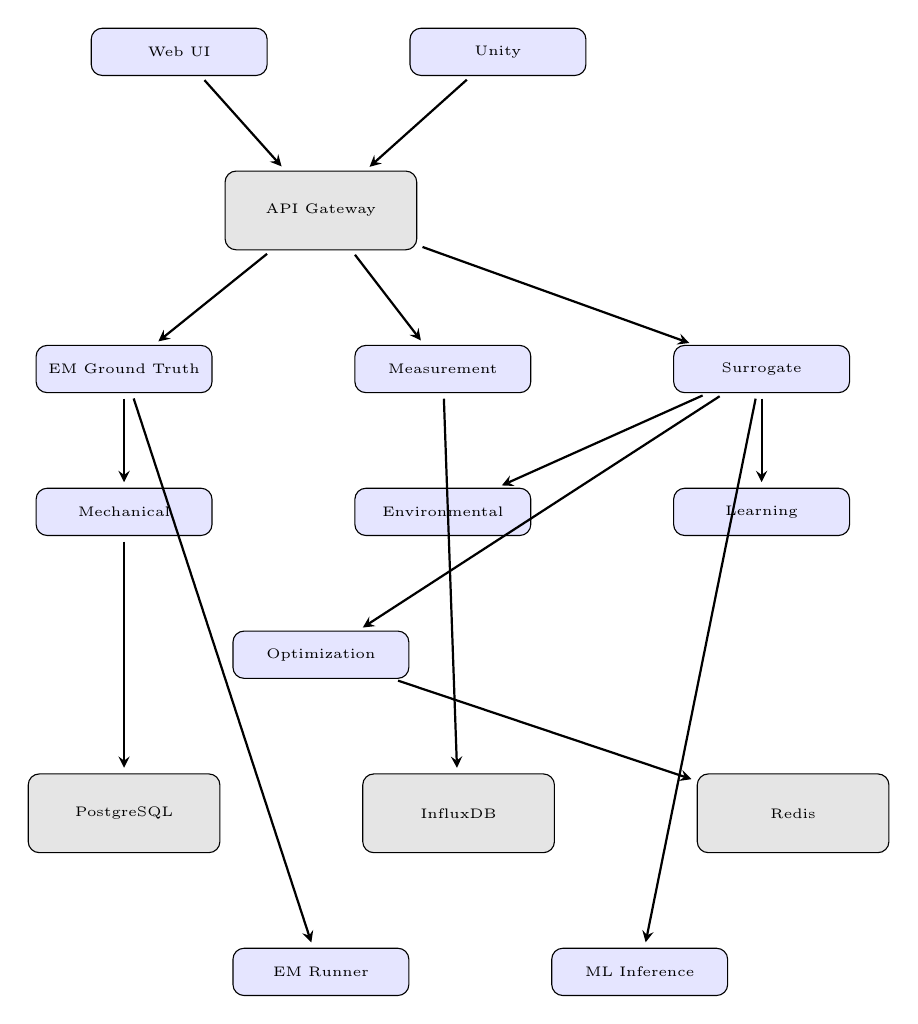
\begin{tikzpicture}[
    node distance=1.2cm and 1.8cm,
    box/.style={rectangle, draw, fill=blue!10, text width=2cm, text centered, minimum height=0.6cm, rounded corners, font=\tiny},
    layer/.style={rectangle, draw, fill=gray!20, text width=2.2cm, text centered, minimum height=1cm, rounded corners, font=\tiny},
    arrow/.style={->, >=stealth, thick, shorten <=2pt, shorten >=2pt}
]
    % Frontend Layer
    \node[box] (webui) {Web UI};
    \node[box, right=of webui] (unity) {Unity};
    
    % API Gateway
    \node[layer, below=of webui, xshift=1.8cm] (api) {API Gateway};
    
    % Core Services
    \node[box, below=of api, xshift=-2.5cm] (em) {EM Ground Truth};
    \node[box, right=of em] (meas) {Measurement};
    \node[box, right=of meas] (surr) {Surrogate};
    \node[box, below=of em] (mech) {Mechanical};
    \node[box, right=of mech] (env) {Environmental};
    \node[box, right=of env] (learn) {Learning};
    \node[box, below=of mech, xshift=2.5cm] (opt) {Optimization};
    
    % Data Layer
    \node[layer, below=of opt, xshift=-2.5cm] (pg) {PostgreSQL};
    \node[layer, right=of pg] (influx) {InfluxDB};
    \node[layer, right=of influx] (redis) {Redis};
    
    % Compute Layer
    \node[box, below=of pg, xshift=2.5cm] (emrun) {EM Runner};
    \node[box, right=of emrun] (ml) {ML Inference};
    
    % Connections
    \draw[arrow] (webui) -- (api);
    \draw[arrow] (unity) -- (api);
    \draw[arrow] (api) -- (em);
    \draw[arrow] (api) -- (meas);
    \draw[arrow] (api) -- (surr);
    \draw[arrow] (em) -- (mech);
    \draw[arrow] (surr) -- (env);
    \draw[arrow] (surr) -- (learn);
    \draw[arrow] (surr) -- (opt);
    \draw[arrow] (mech) -- (pg);
    \draw[arrow] (meas) -- (influx);
    \draw[arrow] (opt) -- (redis);
    \draw[arrow] (em) -- (emrun);
    \draw[arrow] (surr) -- (ml);
\end{tikzpicture}
}
\caption{Proposed Antenna Digital Twin System Architecture}
\label{fig:system_arch}
\end{figure}

\section{Implementation Plan}

The implementation will follow an 11-phase approach to ensure systematic development:

\textbf{Phase 0: Foundation \& Scope Lock} - We will establish project architecture, define frozen scope parameters (rectangular patch, single-band, 2.4/3.5 GHz), and set up modular project structure with backend, frontend, and Unity components.

\textbf{Phase 1: EM Ground Truth Module} - We will develop a solver-agnostic interface supporting multiple EM solvers (Meep, OpenEMS, HFSS, CST, FEKO), implement Design of Experiments (DoE) using Latin Hypercube Sampling, and create batch simulation runners for parallel execution.

\textbf{Phase 2: Measurement Ingestion} - We will develop the software infrastructure for measurement data ingestion, including parsers for standard VNA and chamber measurement file formats (Touchstone, CSV, JSON), implement data validation and quality scoring algorithms, and integrate time-series storage using InfluxDB. The system will be designed to automatically ingest and process measurement data when available, and can be tested using sample measurement files during development.

\textbf{Phase 3: Reduced-Order Modeling} - We will implement sensitivity analysis using Sobol indices and Morris screening to identify critical parameters, and apply dimensionality reduction techniques for optimization efficiency.

\textbf{Phase 4: Surrogate Intelligence Layer} - We will train ensemble surrogate models combining Gaussian Process regression (for uncertainty quantification) and neural networks (for fast inference), targeting prediction accuracy within 1 dB MAE with 95\% confidence intervals.

\textbf{Phase 5: Mechanical Twin} - We will model physical deformations including substrate bending, stress effects, and thermal expansion to predict performance under mechanical loading.

\textbf{Phase 6: Environmental Layer} - We will implement models for orientation effects, proximity interactions (hand, housing), and propagation environments to provide realistic performance predictions.

\textbf{Phase 7: Closed-Loop Learning} - We will develop Bayesian model updating mechanisms to incorporate measurement data, implement drift detection, and create automated retraining pipelines.

\textbf{Phase 8: Optimization Engine} - We will implement geometry optimization algorithms (L-BFGS-B, Differential Evolution) for target performance metrics, and provide what-if analysis capabilities.

\textbf{Phase 9: Unity Visualization} - We will develop Unity-based 3D visualization components for interactive virtual twin representation, including radiation pattern visualization and coverage mapping.

\textbf{Phase 10: Validation Layer} - We will implement validation frameworks to compare surrogate predictions with full EM simulations, and track performance metrics (accuracy, latency, uncertainty calibration).

\textbf{Phase 11: Production Architecture} - We will deploy the system using Docker Compose with service orchestration (PostgreSQL, InfluxDB, Redis), and prepare for scalable cloud deployment.

\subsection{Validation and Testing}
All phases described above involve software development that can be completed and tested using simulated or sample data. Hardware validation and testing with actual lab equipment (VNA, anechoic chamber) will be conducted as a separate validation phase after the software development is complete. This validation will verify the system's performance with real-world measurement data and ensure the closed-loop learning mechanisms work effectively with physical antenna measurements.

\section{Expected Outcomes}

Upon completion, the platform is expected to achieve:
\begin{itemize}
    \item \textbf{Performance:} Real-time predictions (target: $<$10ms) compared to hours for full EM simulation
    \item \textbf{Accuracy:} Mean Absolute Error $<$ 1 dB for S11 predictions with well-calibrated uncertainty bounds
    \item \textbf{Scalability:} Support for 1000+ training samples and extensible to multiple antenna types
    \item \textbf{Integration:} Seamless workflow from EM simulation through ML prediction to measurement validation
\end{itemize}

\section{Technical Approach}

\subsection{Machine Learning Framework}
We will employ an ensemble approach combining Gaussian Process regression and neural networks. The GP model will provide uncertainty quantification using Matern kernels, while the neural network will enable fast inference. The ensemble will fuse predictions using weighted averaging based on validation performance.

\subsection{Technology Stack}
The platform will be built using Python 3.11+ (backend), React + TypeScript (frontend), FastAPI (REST API), PostgreSQL/InfluxDB (databases), and Unity (3D visualization). The system will be containerized using Docker Compose for easy deployment.

\section{Conclusion}

This proposal outlines a comprehensive approach to developing an Antenna Digital Twin platform that will bridge the gap between high-fidelity EM simulation and rapid design iteration. The 11-phase implementation strategy ensures systematic development while maintaining modularity and extensibility. Upon completion, the platform will enable real-time predictions, optimization, and continuous improvement from measurement data, significantly accelerating antenna design workflows.

\section*{References}
\begin{enumerate}
    \item D. M. Pozar, ``Microstrip antennas,'' \emph{Proceedings of the IEEE}, vol. 80, no. 1, pp. 79--91, 1992.
    \item C. E. Rasmussen and C. K. I. Williams, \emph{Gaussian Processes for Machine Learning}. Cambridge, MA, USA: MIT Press, 2006.
    \item C. A. Balanis, \emph{Antenna Theory: Analysis and Design}, 4th ed. Hoboken, NJ, USA: Wiley, 2016.
    \item A. Saltelli et al., \emph{Global Sensitivity Analysis: The Primer}. Chichester, UK: Wiley, 2008.
    \item Altair FEKO, ``High-frequency electromagnetic simulation software,'' \url{https://altair.com/feko}, accessed Dec. 2025.
\end{enumerate}

\end{document}
